%-------------------------------------------------------------------------------

% This file is part of Code_Saturne, a general-purpose CFD tool.
%
% Copyright (C) 1998-2016 EDF S.A.
%
% This program is free software; you can redistribute it and/or modify it under
% the terms of the GNU General Public License as published by the Free Software
% Foundation; either version 2 of the License, or (at your option) any later
% version.
%
% This program is distributed in the hope that it will be useful, but WITHOUT
% ANY WARRANTY; without even the implied warranty of MERCHANTABILITY or FITNESS
% FOR A PARTICULAR PURPOSE.  See the GNU General Public License for more
% details.
%
% You should have received a copy of the GNU General Public License along with
% this program; if not, write to the Free Software Foundation, Inc., 51 Franklin
% Street, Fifth Floor, Boston, MA 02110-1301, USA.

%-------------------------------------------------------------------------------

\programme{clptur}

\vspace{1cm}
%%%%%%%%%%%%%%%%%%%%%%%%%%%%%%%%%%
%%%%%%%%%%%%%%%%%%%%%%%%%%%%%%%%%%
\section*{Function}
%%%%%%%%%%%%%%%%%%%%%%%%%%%%%%%%%%
%%%%%%%%%%%%%%%%%%%%%%%%%%%%%%%%%%
This subroutine is dedicated to the calculation of the wall boundary conditions. The notations introduced in \var{CONDLI} for the general boundary conditions will be used.

The wall boundary conditions refer to all the boundary conditions for the velocity, the turbulent variables ($k$, $\varepsilon$, $R_{ij}$), the temperature when it has a prescribed value at the wall (or the enthalpy and more generally the {\it VarScalaires}\footnote{As in \fort{condli} the {\it VarScalaire} are any solution of a convection-diffusion equation apart from the velocity, the pressure and the turbulent variables  $k$, $\varepsilon$ and $R_{ij}$. More specifically, the name {\it VarScalaire} can refer to the temperature, the enthalpy or a passive scalar.  } to treat at the wall by using a similarity law for the associated boundary layer). For the {\it VarScalaire} in particular, when the boundary conditions at the wall are of Neumann type (homogeneous or not), they are treated in  \fort{condli} and don't present them here. In particular, the boundary conditions of the {\it VarScalaires} are not treated here because their treatment at the wall is of homogeneous Neumann type.

We present the calculation of the pair of coefficients $A_b$ and $B_b$ which are used during the computation of certain discretized terms of the equations to solve, and which allow in particular to determine a value associated with the boundary faces $f_{b,int}$ (at a point located at the "centre" of the boundary face, the barycentre of its vertices) using the formulae   $f_{b,int} = A_b+B_b\,f_{I'}$ ($f_{I'}$ is the value of the variable at point $I'$, the projection of the centre of the boundary cell onto the line normal to the boundary face and passing through its centre~: see figure~\ref{Base_Clptur_fig_flux_clptur}).


\begin{figure}[h]
\centerline{\includegraphics[height=7cm]{fluxbord}}
\caption{\label{Base_Clptur_fig_flux_clptur}Boundary cell.}
\end{figure}

%%%%%%%%%%%%%%%%%%%%%%%%%%%%%%%%%%
%%%%%%%%%%%%%%%%%%%%%%%%%%%%%%%%%%
\section*{Discretisation}
%%%%%%%%%%%%%%%%%%%%%%%%%%%%%%%%%%
%%%%%%%%%%%%%%%%%%%%%%%%%%%%%%%%%%

\etape{Notations\vspace{0,3cm}}
%%%%%%%%%%%%%%%%%%%%%%%%%%%%%%%%%%%%%%%%%%%%%%%%%%%%%%%%%%%%%%%%%%%%%%%%%%%%%%%
The velocity of the wall is noted
$\vect{v}_p$. We assume it is projected onto the plane tangent to the wall (if it is not, then the code projects it).


The velocity of the fluid is noted $\vect{u}$. Index $I$, $I'$ or $F$ denotes the point at which the velocity is estimated. The component tangent to the wall writes $u_\tau$. The fluid velocity in the coordinate system attached to the wall ("relative" velocity) writes $\vect{u}^r=\vect{u} - \vect{v}_p$.



The orthonormal coordinate system attached to the wall writes
$\hat {\mathcal R}=(\vect{\tau},\vect{\tilde{n}},\vect{b})$.
\begin{itemize}
\item [$\bullet$] $\vect{\tilde{n}}=-\vect{n}$ is the unit vector orthogonal to the wall and directed towards the interior of the computational domain.
\item [$\bullet$] $\vect{\tau} = \displaystyle\frac{1}{\|\vect{u}^r_{I'}-(\vect{u}^r_{I'}\,.\,\vect{\tilde{n}})\|}\left[\vect{u}^r_{I'}-(\vect{u}^r_{I'}\,.\,\vect{\tilde{n}})\right]$ is the unit vector parallel to the projection of the relative velocity at $I'$, $\vect{u}^r_{I'}$, in the plane tangent to the wall
 ({\it i.e.} orthogonal to $\vect{\tilde{n}}$)~: see
figure~\ref{Base_Clptur_fig_flux_clptur}.
\item [$\bullet$] $\vect{b}$ is the unit vector which completes the positively oriented coordinate system.
\end{itemize}
\vspace{0.2cm}

The dimensionless limit distance which separates the viscous sublayer from the logarithmic region writes $y^+_{lim}$. Its value is $1/\kappa$ (with $\kappa = 0,42$) in general (to ensure the continuity of the velocity gradient) and 10.88 in LES (to ensure the continuity of the velocity).

In the case of the {\bf two velocity scale model},
\begin{itemize}
\item [-] $u_k$ is the friction velocity at the wall obtained from the turbulent kinetic energy.
We write $u^*$ the friction velocity at the wall calculated from the equation
 $ \displaystyle\frac{u^r_{\tau,I'}}{u^*} = f(y^+_k)$.

\item [-]
$y^+_k$  represents a dimensionless wall distance,
$y^+_k= \displaystyle\frac{u_k\,I'F}{\nu}$ ($\nu$ is the molecular kinematic viscosity
taken at the centre $I$ of the boundary cell).
The function $f$ gives the ideal shape of the velocity profile.
It is piecewisely approximated by the logarithmic law
 $f(z)=f_1(z)= \displaystyle\frac{1}{\kappa}ln(z)+5,2$ for
$z> y^+_{lim}$
and by the linear law $f(z)=f_2(z)=z$ otherwise.

\item [-] The two velocity scale $u_k$ and $u^*$ are simple to compute
but their computation requires the knowledge of the turbulent kinetic energy $k_I$
at the centre of cell adjoint to the boundary face  (with the $R_{ij}-\varepsilon$ model, we use half the trace of the Reynolds stress tensor).


\item [-] The two velocity scale model is the default model in \CS.
It often permits, and in particular in cases with heat transfer, to reduce the
effects of certain flaws associated to the $k-\varepsilon$ model.
\end{itemize}


Later on, we will use $u^*$ and $u_k$ for the boundary conditions of the velocity and scalars (in particular the temperature).


\begin{equation}\label{Base_Clptur_Eq_Mod_'2ech_Vit}
\begin{array}{l}
\text{\bf Two velocity scale model}\\
\left\{\begin{array}{l}
u_k = C_\mu^\frac{1}{4}k_I^\frac{1}{2}\\
u^* \text{is solution of }
\left\{\begin{array}{lll}
\displaystyle\frac{u^r_{\tau,I'}}{u^*} &=
\displaystyle\frac{1}{\kappa}ln(y^+_k)+5,2 &\text { for }y^+_k>y^+_{lim}\\
\displaystyle\frac{u^r_{\tau,I'}}{u^*} &= y^+_k                &\text { for }
y^+_k \leqslant y^+_{lim}
\end{array}\right.    \\
\qquad\qquad
\text{   with   } C_\mu =0,09\qquad y^+_k=\displaystyle\frac{u_k\,I'F}{\nu}
                                                      \text{  and }\kappa = 0,42
\end{array}\right.
\end{array}
\end{equation}



In the case of the {\bf one velocity scale model},

we write $u^*$ the only
friction velocity at the wall solution of the equation
$\displaystyle\frac{u^r_{\tau,I'}}{u^*} = f(y^+)$.
$y^+$  represents a dimensionless wall distance
$y^+=\displaystyle\frac{u^*\,I'F}{\nu}$ ($\nu$ is the molecular kinematic viscosity
taken at the centre $I$ of the boundary cell).
The function $f$ gives the ideal shape of the velocity profile, as in the case of the two velocity scale model. One can note that this friction velocity, calculated using a more complicated approach (Newton method), can however be obtained without making any reference to the turbulent variables ($k$, $\varepsilon$, $R_{ij}$). For convenience in the case of the one velocity scale model, we write $u_k=u^*$.

Later on, we will use $u^*$ and $u_k$ for the boundary conditions of the velocity and scalars (in particular the temperature).

\begin{equation}
\begin{array}{l}
\text{\bf Mod\`ele \`a une \'echelle de vitesse}\\
\left\{\begin{array}{l}
u_k = u^*\\
u^* \text{ solution de } \left\{\begin{array}{lll}
\displaystyle\frac{u^r_{\tau,I'}}{u^*} &=
\displaystyle\frac{1}{\kappa}ln(y^+)+5,2 &\text { pour }y^+>y^+_{lim}\\
\displaystyle\frac{u^r_{\tau,I'}}{u^*} &= y^+                         &\text
{pour } y^+\leqslant y^+_{lim}
\end{array}\right.\\
\qquad\qquad\text{   avec   } y^+=\displaystyle\frac{u^*\,I'F}{\nu}
                                                      \text{  et }\kappa=0,42
\end{array}\right.
\end{array}
\end{equation}


{\bf Remark~:} Hereafter, we provide three exemples
based on the two velocity scale model.
\begin{itemize}
\item In this way, one can implement a specific wall function~:
$$\displaystyle\frac{u_{\tau,I'}}{u^*}=g(y^+)$$
by simply imposing
$\displaystyle{u^*}=u_{\tau,I'}/g(y^+)$.
\item It is also possible to use a rough-wall wall function such as~:
$$\displaystyle\frac{u_{\tau,I'}}{u^*}=\displaystyle\frac{1}{\kappa}\,ln(\frac{y}{\xi})+8,5$$
where $\xi$ is the height of the roughness elements at the wall~: one just has to impose
$\displaystyle u^*=u_{\tau,I'}/\left[\frac{1}{\kappa}ln(\frac{y}{\xi})+8,5\right]$,
 $y$ being deduced from $y^+$, available as an argument, by the equation
$\displaystyle y=y^+\frac{\nu}{u_k}$.
\item Even a more general correlation could be used of
Colebrook type~:
$$u^*=u_{deb}/\left[-4\sqrt{2}log_{10}\left(\displaystyle\frac{2,51}{2\sqrt{2}D_H^+}+\frac{\xi}{3,7\,D_H}\right)\right]$$
where $D_H^+$ is the hydraulic diameter made dimensionless using $u_k$, $\nu$,
$u_{deb}$ the mean streamwise velocity
and $\displaystyle\frac{\xi}{D_H}$ the relative roughness.
\end{itemize}



\etape{Boundary conditions for the velocity in $k-\varepsilon$\vspace{0,3cm}}
%%%%%%%%%%%%%%%%%%%%%%%%%%%%%%%%%%%%%%%%%%%%%%%%%%%%%%%%%%%%%%%%%%%%%%%%%%%%%%%
We first consider the boundary conditions used in the case of calculation using the
 $k-\varepsilon$ model. Indeed these cases are the most complex and general.

The boundary conditions are necessary to prescribe at the boundary
 the correct tangential stress $\sigma_\tau=\rho_Iu^*u_k$ in the momentum
equation\footnote{Proposition de modification des conditions aux limites de
paroi turbulente pour le Solveur Commun dans le cadre du mod\`ele
$k-\varepsilon$ standard, rapport EDF HI-81/00/019/A, 2000, M. Boucker, J.-D. Mattei.}
($\rho_I$ is the density at the centre of cell $I$).
The term which requires boundary conditions is the one containing the
velocity derivative in the normal direction to the wall\footnote{The transpose gradient term is treated in \fort{visecv}
and thus will not be considered here.}~:
$(\mu_I+\mu_{t,I})\ggrad{\vect{u}}\,\vect{n}$. It appears on the
right-hand side of the usual momentum equation (see \fort{bilsc2} and \fort{predvv}).

In the case where the  $k-\varepsilon$  model tends to surestimate
the production of turbulent kinetic energy, the length scale of the model,
$L_{k-\varepsilon}$,
can become significantly larger than the maximum theoretical length scale
of the turbulent boundary layer eddies  $L_{\text{theo}}$. We write~:
\begin{equation}
\left\{\begin{array}{l}
L_{k-\varepsilon} = C_{\mu}\displaystyle\frac{k^\frac{3}{2}}{\varepsilon}\\
L_{\text{theo}} = \kappa\, I'F
\end{array}\right.
\end{equation}

In the case where $L_{k-\varepsilon}>L_{\text{th\'eo}}$, we thus have
$\mu_{t,I}>\mu_{t}^{lm}$ with $\mu_{t,I}$ the turbulent viscosity of the
$k-\varepsilon$ model at point $I$ and $\mu_{t}^{lm}=\rho_I L_{\text{theo}}u_k$
the turbulent viscosity of the mixing length model. Additionally, the
tangential stress can write by making the turbulent viscosity appear~:
\begin{equation}
\sigma_\tau = \rho_Iu^*u_k = \displaystyle\frac{u^*}{\kappa\, I'F}\underbrace{\rho_I\kappa\, I'F\, u_k}_{\mu^{lm}_t}
\end{equation}
The viscosity scale introduced in the stress thus contradicts the one deduced
from the neighbouring turbulence calculated by the model.
Consequently we prefer to write the stress, by using the velocity scale of the $k-\varepsilon$ model when it is lower than
the limit $L_{\text{th\'eo}}$~:
\begin{equation}
\sigma_\tau = \displaystyle\frac{u^*}{\kappa\, I'F} max(\mu_{t}^{lm},\mu_{t,I})
\end{equation}

One can then use this value to calculate the diffusive flux
which depends upon it in the Navier-Stokes equations~:
\begin{equation}\label{Base_Clptur_eq_grad_sigma_clptur}
(\mu_I+\mu_{t,I})\ggrad{\vect{u}}\,\vect{n}=-\sigma_\tau \vect{\tau}.
\end{equation}

But the velocity gradient (face gradient) is computed in the code as~:
\begin{equation}\label{Base_Clptur_eq_grad_uf_clptur}
(\mu_I+\mu_{t,I})\ggrad{\vect{u}}\,\vect{n}=
\displaystyle\frac{(\mu_I+\mu_{t,I})}{\overline{I'F}}(\vect{u}_F-\vect{u}_{I'})
\end{equation}

Using (\ref{Base_Clptur_eq_grad_sigma_clptur}) and
(\ref{Base_Clptur_eq_grad_uf_clptur}) we obtain the value of $\vect{u}_F$
to be prescribed, referred to as $\vect{u}_{F,flux}$~(conservation of the momentum flux)~:
\begin{equation}\label{Base_Clptur_eq_uf_flux_clptur}
\begin{array}{ll}
\vect{u}_{F,flux}&=\vect{u}_{I'}-\displaystyle\frac{\overline{I'F}}{\mu_I+\mu_{t,I}}\sigma_\tau \vect{\tau}\\
                 &=\vect{u}_{I'}-\displaystyle\frac{u^*}{\kappa\, (\mu_I+\mu_{t,I})} max(\mu_{t}^{lm},\mu_{t,I}) \vect{\tau}
\end{array}
\end{equation}

In reality, an extra approximation is made. It consists in imposing a zero
 normal velocity at the wall and in using equation (\ref{Base_Clptur_eq_uf_flux_clptur})
 projected on the plane parallel to the wall~:
\begin{equation}
\vect{u}_{F,flux}=\left[u_{\tau,I'}-\displaystyle\frac{u^*}{\kappa\,
(\mu_I+\mu_{t,I})} max(\mu_{t}^{lm},\mu_{t,I}) \right]\vect{\tau}
\end{equation}

Moreover, if the value obtained for $y^+$ is
lower than  $y^+_{lim}$ a no-slip condition is applied.
Finally, one can also make the wall velocity appear in the final expression~:
\begin{equation}
\begin{array}{l}
\text{\bf "Flux" boundary conditions of the velocity}\,(k-\varepsilon)\\
\left\{\begin{array}{llr}
\vect{u}_{F,flux}&=\vect{v}_p& \text{ if\ }  y^+\leqslant
                           y^+_{lim} \\
\vect{u}_{F,flux}&=\vect{v}_p+&\left[u^r_{\tau,I'}-\displaystyle\frac{u^*}{\kappa\,
(\mu_I+\mu_{t,I})} max(\mu_{t}^{lm},\mu_{t,I}) \right]\vect{\tau}
\text{ otherwise }
\end{array}\right.
\end{array}
\end{equation}

A first pair of coefficients $A_{flux}$ and $B_{flux}$ can then be deduced
(for each component of the velocity separately) and it is used only
 to compute the tangential stress dependent term  (see \fort{bilsc2})~:
\begin{equation}
\begin{array}{l}
\text{\bf Coefficients associated with  the "flux" boundary conditions of the velocity } (k-\varepsilon)\\
\left\{\begin{array}{l}
\left\{\begin{array}{llr}
\vect{A}_{flux}&=\vect{v}_p& \text{ if\ } y^+\leqslant y^+_{lim} \\
\vect{A}_{flux}&=\vect{v}_p+&\left[u^r_{\tau,I'}-\displaystyle\frac{u^*}{\kappa\,
(\mu_I+\mu_{t,I})} max(\mu_{t}^{lm},\mu_{t,I}) \right]\vect{\tau} \text{ otherwise }
\end{array}\right.  \\
\vect{B}_{flux} = \vect{0}
\end{array}\right.
\end{array}
\end{equation}

We saw above how to impose a boundary condition to compute directly the stress term.
Further analysis is necessary to calculate correctly the velocity gradients. We
want to find a boundary face value which permits to obtain,
with the chosen expression for the gradient,
 the value the turbulent production as close as possible to its theoretical value
(determined by using the logarithmic law), in order to evaluate the normal
derivative the tangential velocity.
Thus, we define (at point $I$)~:
\begin{equation}\label{Base_Clptur_eq_ptheo_clptur}
P_{\text{th\'eo}} = \rho_I u^* u_k
\|\displaystyle\frac{\partial u_\tau}{\partial\vect{n}}\|_{I} =
\rho_I \displaystyle\frac{u_k(u^*)^2}{\kappa\, I'F}
\end{equation}

Morevoer, the dominant term of the production computed in cell $I$ is,
in classical situations ($y$ is the coordinate on the axis
whose direction vector is $\vect{\tilde{n}}$),
\begin{equation}
P_{\text{calc}} =
\mu_{t,I}\left(\displaystyle\frac{\partial u_\tau}{\partial y}\right)^2_{I}
\end{equation}

The normal gradient of the tangential velocity (cell gradient)
is calculated in the code using finite volume, and its expression
on regular orthogonal meshes is (see the notations on
figure \ref{Base_Clptur_fig_bord_ortho_clptur})~:
\begin{equation}
P_{\text{calc}} =
\mu_{t,I}\left(\displaystyle\frac{u_{\tau,G}-u_{\tau,F}}{2d}\right)^2 =
\mu_{t,I}\left(\displaystyle\frac{u_{\tau,I}+u_{\tau,J}-2u_{\tau,F}}{4d}\right)^2
\end{equation}
We then assume that $u_{\tau,J}$ can be obtained from $u_{\tau,I}$
and from the normal gradient of $u_{\tau}$ calculated in G
from the logarithmic law~:
\begin{equation}
\label{Base_Clptur_eq_dvp_lim_utau}
u_{\tau,J}=u_{\tau,I}+ IJ\,.\,(\partial_y u_{\tau})_G+\mathcal{O} (IJ^{\,2}) \approx
u_{\tau,I}+ IJ\,.\,\left[\partial_y \left(\displaystyle
\frac{u^*}{\kappa}\,ln{ (y^+)} + 5,2 \right)\right]_G=
u_{\tau,I}+2d\displaystyle\frac{u^*}{\kappa\, 2d}
\end{equation}
and thus we obtain~:
\begin{equation}\label{Base_Clptur_eq_pcalc_clptur}
\begin{array}{lll}
P_{\text{calc}} &=&
\mu_{t,I}\left(\displaystyle\frac{u_{\tau,I}+u_{\tau,I}+2d\frac{u^*}{\kappa\, 2d}-2u_{\tau,F}}{4d}\right)^2 \\
&=&\mu_{t,I}\left(\displaystyle\frac{2u_{\tau,I}+2\frac{u^*}{2\kappa}-2u_{\tau,F}}{4d}\right)^2 =
\mu_{t,I}\left(\displaystyle\frac{u_{\tau,I}+\frac{u^*}{2\kappa}-u_{\tau,F}}{2d}\right)^2
\end{array}
\end{equation}

\begin{figure}[h]
\centerline{\includegraphics[height=7cm]{bordortho}}
\caption{\label{Base_Clptur_fig_bord_ortho_clptur}Cellule de bord - Maillage orthogonal.}
\end{figure}

We then use (\ref{Base_Clptur_eq_ptheo_clptur}) and
(\ref{Base_Clptur_eq_pcalc_clptur}) to impose that the calculated
production is equal to the theoretical production. The preceeding
formulae are extended with no precaution to non-orthogonal meshes (the velocity
at $I$ is then simply computed at $I'$).
The following expression for $u_{\tau,F}$ is then obtained~:
\begin{equation}
u_{\tau,F,grad} =u_{\tau,I'}-\displaystyle\frac{u^*}{\kappa}\left(
2\sqrt{\displaystyle\frac{\rho_I\kappa\, u_k I'F}{\mu_{t,I}} }-\displaystyle\frac{1}{2}\right)
\end{equation}

Additionally, we force the gradient to remain as stiff as the one
given by the normal derivative of the theoretical velocity profile
(logarithmic) at $I'$~:\\
$\partial_y u_{\tau} = \partial_y (\displaystyle
\frac{u^*}{\kappa}\,ln{ (y^+)} + 5,2 ) =\displaystyle\frac{u^*}{\kappa\, \overline{I'F}}$, thus~:
\begin{equation}
u_{\tau,F,grad} =u_{\tau,I'}-\displaystyle\frac{u^*}{\kappa}max\left(1,
2\sqrt{\displaystyle\frac{\rho_I\kappa\, u_k I'F}{\mu_{t,I}} }-\displaystyle\frac{1}{2}\right)
\end{equation}

Finally, we clip the velocity at the wall with a minimum value calculated
assuming that we are in the logarithmic layer~:
\begin{equation}\label{Base_Clptur_eq_ugrad_clptur}
u_{\tau,F,grad} =
max\left(u^*\left(\displaystyle\frac{1}{\kappa}ln(y^+_{lim})+5,2\right),
u_{\tau,I'}-\displaystyle\frac{u^*}{\kappa}\left[max\left(1,
2\sqrt{\displaystyle\frac{\rho_I\kappa\, u_k I'F}{\mu_{t,I}}
}-\displaystyle\frac{1}{2}\right)\right]\right)
\end{equation}


The normal derivative at the wall is prescribed to zero.
If the $y^+$ value at the wall is lower than  $y^+_{lim}$,
a no-slip condition is prescribed. Finally, one can also
make explicit the velocity of the wall in the final expression~:
\begin{equation}
\begin{array}{l}
\text{\bf "Gradient" boundary conditions of the velocity} (k-\varepsilon)\\
\left\{\begin{array}{l}
\vect{u}_{F,grad}=\vect{v}_p
          \qquad\qquad\text{ if }  y^+\leqslant y^+_{lim} \\
\vect{u}_{F,grad}=\vect{v}_p+\\
          \left\{
max\left(u^*\left(\displaystyle\frac{1}{\kappa}ln(y^+_{lim})+5,2\right),
u^r_{\tau,I'}-\displaystyle\frac{u^*}{\kappa}\left[max\left(1,
2\sqrt{\displaystyle\frac{\rho_I\kappa\, u_k I'F}{\mu_{t,I}}
}-\displaystyle\frac{1}{2}\right)\right]\right)
\right\}\vect{\tau}
          \text{ otherwise }
\end{array}\right.
\end{array}
\end{equation}

A second pair of coefficients $A_{grad}$ and $B_{grad}$ can then be deduced
(for each velocity component separately). It is used when the velocity
gradient is necessary (except for the terms depending on the tangential shear,
those being treated in \fort{bilsc2} using $A_{flux}$ and $B_{flux}$)~:
\begin{equation}
\begin{array}{l}
\text{\bf Coefficients associated to the "gradient" boundary conditions of }\\
\qquad\qquad\qquad\qquad\text{\bf the velocity}  (k-\varepsilon)\\
\left\{\begin{array}{l}
\left\{\begin{array}{l}
\vect{A}_{grad}=\vect{v}_p
                    \qquad\qquad\text{ \ if\ } y^+\leqslant y^+_{lim} \\
\vect{A}_{grad}=\vect{v}_p+\\
\left\{
max\left(u^*\left(\displaystyle\frac{1}{\kappa}ln(y^+_{lim})+5,2\right),
u^r_{\tau,I'}-\displaystyle\frac{u^*}{\kappa}\left[max\left(1,
2\sqrt{\displaystyle\frac{\rho_I\kappa\, u_k I'F}{\mu_{t,I}}
}-\displaystyle\frac{1}{2}\right)\right]\right)
\right\}\vect{\tau}
    \text{ otherwise }
\end{array}\right.  \\
\vect{B}_{grad} = \vect{0}
\end{array}\right.
\end{array}
\end{equation}


\etape{Boundary conditions of the velocity in $R_{ij}-\varepsilon$\vspace{0,3cm}}
%%%%%%%%%%%%%%%%%%%%%%%%%%%%%%%%%%%%%%%%%%%%%%%%%%%%%%%%%%%%%%%%%%%%%%%%%%%%%%%
The boundary conditions of the velocity with the  $R_{ij}-\varepsilon$ model are
more simple, since there are only of one type.
Keeping the same notations as above, we want the tangential velocity gradient
(calculated at $I$, and to be used to evaluate the turbulent production)
to be consistent with the logarithmic law giving the ideal tangential
velocity profile. The theoretical gradient is~:

\begin{equation}\label{Base_Clptur_eq_grad_theo_clptur}
G_{\text{theo}} = \left(\displaystyle\frac{\partial u_\tau}{\partial y}\right)_{I'}=\frac{u^*}{\kappa\, I'F}
\end{equation}

The normal gradient of the tangential velocity (cell gradient) is
calculated in the code using finite volumes, and its expression in the case
of regular orthogonal meshes is (see notations in figure
\ref{Base_Clptur_fig_bord_ortho_clptur})~:
\begin{equation}
G_{\text{calc}}=\displaystyle\frac{u_{\tau,G}-u_{\tau,F}}{2d} =
\displaystyle\frac{u_{\tau,I}+u_{\tau,J}-2u_{\tau,F}}{4d}
\end{equation}
We then assume that $u_{\tau,J}$ can be obtained from $u_{\tau,I}$
and from the normal gradient of $u_{\tau}$ calculated in G
from the logarithmic law (see equation (\ref{Base_Clptur_eq_dvp_lim_utau}))
$u_{\tau,J}=u_{\tau,I}+2d\displaystyle\frac{u^*}{\kappa\, 2d}$ and we thus
obtain~:
\begin{equation}\label{Base_Clptur_eq_grad_calc_clptur}
G_{\text{calc}}=\displaystyle\frac{u_{\tau,I}+u_{\tau,I}+2d\displaystyle\frac{u^*}{\kappa\, 2d}-2u_{\tau,F}}{4d}=
\displaystyle\frac{2u_{\tau,I}+2\displaystyle\frac{u^*}{2\kappa}-2u_{\tau,F}}{4d}=
\displaystyle\frac{u_{\tau,I}+\displaystyle\frac{u^*}{2\kappa}-u_{\tau,F}}{2d}
\end{equation}
We then use the equations (\ref{Base_Clptur_eq_grad_theo_clptur}) and
(\ref{Base_Clptur_eq_grad_calc_clptur}) to derive an expression for
$u_{\tau,F}$ (the preceeding
formulae are extended with no precaution to the case non-orthogonal meshes,
the velocity at $I$ being simply computed at $I'$)~:
\begin{equation}
u_{\tau,F}= u_{\tau,I'}-\displaystyle\frac{3u^*}{2\kappa }
\end{equation}
The normal derivative at the wall is prescribed to zero.
If the value obtained for $y^+$ at the wall is lower than  $y^+_{lim}$,
a no-slip condition is prescribed. Finally, one can also
make explicit the velocity of the wall in the final expression~:
\begin{equation}\label{Base_Clptur_eq_CL_vitesse_rij_clptur}
\begin{array}{l}
\text{\bf Boundary conditions of the velocity }(R_{ij}-\varepsilon)\\
\left\{\begin{array}{lll}
\vect{u}_{F}&=\vect{v}_p& \text{ \ if\ } y^+\leqslant
                           y^+_{lim} \\
\vect{u}_{F}&=\left[u^r_{\tau,I'}-\displaystyle\frac{3u^*}{2\kappa } \right]\vect{\tau} +\vect{v}_p &\text{ otherwise }
\end{array}\right.
\end{array}
\end{equation}


Un couple de coefficients $A$ et $B$ s'en d\'eduit (pour
chaque composante de vitesse s\'epar\'ement)~:
\begin{equation}\label{Base_Clptur_eq_AB_vitesse_rij_clptur}
\begin{array}{l}
\text{\bf Coefficients associ\'es aux conditions aux limites sur la vitesse }(R_{ij}-\varepsilon)\\
\left\{\begin{array}{l}
\left\{\begin{array}{lll}
\vect{A}&=\vect{v}_p& \text{ \ si\ } y^+\leqslant y^+_{lim} \\
\vect{A}&=\left[u^r_{\tau,I'}-\displaystyle\frac{3u^*}{2\kappa } \right]\vect{\tau}
+\vect{v}_p &\text{ sinon }
\end{array}\right.\\
\vect{B}= \vect{0}
\end{array}\right.
\end{array}
\end{equation}
A pair of coefficients $A_{grad}$ and $B_{grad}$ can be deduced
from the above equation
(for each velocity component separately).


\etape{Boundary conditions of the velocity in laminar\vspace{0,3cm}}
When no turbulence model is activated, we implicitly use a one velocity
scale model (there is no turbulent variables to compute  $u_k$), and the same
conditions
\footnote{In other words; the boundary conditions are given by
 (\ref{Base_Clptur_eq_CL_vitesse_rij_clptur}) and
(\ref{Base_Clptur_eq_AB_vitesse_rij_clptur}).}
 as in $R_{ij}-\varepsilon$ are used~: the model degenerates automatically.



\newpage

\etape{Boundary conditions for $k$ and $\varepsilon$ (standard
$k-\varepsilon$ model)\vspace{0,3cm}}

We impose $k$ with a Dirichlet condition using the friction velocity
$u_k$ (see equation~(\ref{Base_Clptur_Eq_Mod_'2ech_Vit})) :
\begin{equation}
k= \displaystyle\frac{u_k^2}{C_\mu^\frac{1}{2}}
\end{equation}

We want to impose the normal derivative of  $\varepsilon$ from
of the following theoretical law
 (see the notations in figure \ref{Base_Clptur_fig_bord_ortho_clptur})~:
\begin{equation}\label{Base_Clptur_eq_partialep_theo_clptur}
G_{\text{theo},\varepsilon} = \displaystyle\frac{\partial \left(u_k^3/(\kappa\, y)\right)}{\partial y}
\end{equation}



We use point $M$ to impose a boundary condition with a higher order of
accuracy in space.
 Indeed, using the simple expression
$\varepsilon_F=\varepsilon_I+d\partial_y\varepsilon_I + O(d^2)$ leads to
first order accuracy.
 A second order accuracy can be reached
 using the following Taylor series expansion:
\begin{equation}
\left\{\begin{array}{ll}
\varepsilon_M&=\varepsilon_I-\displaystyle\frac{d}{2}\partial_y\varepsilon_I+\displaystyle\frac{d^2}{8}\partial^2_y\varepsilon_I+O(d^3)\\
\varepsilon_M&=\varepsilon_F+\displaystyle\frac{d}{2}\partial_y\varepsilon_F+\displaystyle\frac{d^2}{8}\partial^2_y\varepsilon_F+O(d^3)
\end{array}\right.
\end{equation}
By substracting these twxo expression, we obtain
\begin{equation}\label{Base_Clptur_eq_epsf_clptur}
\varepsilon_F=\varepsilon_I-\displaystyle\frac{d}{2}(\partial_y\varepsilon_I+\partial_y\varepsilon_F)+O(d^3)
\end{equation}
Additionally, we have
\begin{equation}
\left\{\begin{array}{ll}
\partial_y\varepsilon_I&=\partial_y\varepsilon_M+d\partial^2_y\varepsilon_M+O(d^2)\\
\partial_y\varepsilon_F&=\partial_y\varepsilon_M-d\partial^2_y\varepsilon_M+O(d^2)
\end{array}\right.
\end{equation}
The sum of these last two expressions gives
$\partial_y\varepsilon_I+\partial_y\varepsilon_F=2\partial_y\varepsilon_M+O(d^2)$ and,
using equation
(\ref{Base_Clptur_eq_epsf_clptur}), we finally obtain a second order
approximation for $\varepsilon_F$~:
\begin{equation}
\varepsilon_F=\varepsilon_I-d\partial_y\varepsilon_M+O(d^3)
\end{equation}
The theoretical value (see equation \ref{Base_Clptur_eq_partialep_theo_clptur})
is then used in order to evaluate
 $\partial_y\varepsilon_M$ and thus the value to prescribe at
the boundary is obtained ($d=I'F$)~:
\begin{equation}
\varepsilon_F=\varepsilon_I+d\displaystyle\frac{ u_k^3}{\kappa\, (d/2)^2}
\end{equation}

This expression is extended to non-orthogonal mesh without any precautions
(which is bound to deteriorate the spatial accuracy ot the method).

Additionally, the velocity $u_k$ is set to zero for $y^+\leqslant y^+_{lim}$.
Consequently, the value of $k$ and the flux of $\varepsilon$ are both zero.

Finally we have~:

\begin{equation}
\begin{array}{l}
\text{\bf Boundary conditions for } k \text { \bf and } \varepsilon \\
\left\{\begin{array}{ll}
k_F&= \displaystyle\frac{u_k^2}{C_\mu^\frac{1}{2}}\\
\varepsilon_F&=\varepsilon_{I'}+I'F\displaystyle\frac{ u_k^3}{\kappa\, (I'F/2)^2}
\end{array}\right. \\
\text{with } u_k = 0 \text { if } y^+\leqslant y^+_{lim}
\end{array}
\end{equation}
and the associated pair of coefficients
\begin{equation}
\begin{array}{l}
\text{\bf Coefficients associated to the boundary conditions of }
k \text { \bf et } \varepsilon \\
\left\{\begin{array}{llll}
A_k&= \displaystyle\frac{u_k^2}{C_\mu^\frac{1}{2}} &\text{ and } B_k&= 0 \\
A_\varepsilon&=I'F\displaystyle\frac{ u_k^3}{\kappa\, (I'F/2)^2}&\text{ and } B_\varepsilon&= 1
\end{array}\right.\\
\text{with } u_k = 0 \text { if } y^+\leqslant y^+_{lim}
\end{array}
\end{equation}







\etape{Boundary conditions for $R_{ij}$ and $\varepsilon$
(standard $R_{ij}-\varepsilon$ model)\vspace{0,3cm}}

The boundary conditions for the Reynolds stresses in the coordinate system
attached to the wall write ($\hat R$ refers to the local coordinate system)~:
\begin{equation}
\begin{array}{lll}
\partial_{\tilde{n}} \hat R_{\tau\tau} = \partial_{\tilde{n}} \hat R_{\tilde{n}\tilde{n}}=\partial_{\tilde{n}} \hat R_{bb}=0  &
\text { et } \hat R_{\tau\tilde{n}} = -u^*u_k  &\text { et  } \hat R_{\tau b} = \hat R_{\tilde{n} b}
= 0
\end{array}
\end{equation}


Additionally, if the value obtained for $y^+$ is lower
than  $y^+_{lim}$, all Reynolds stresses are set to zero
(we assume that the turbulent stresses are negligible
compared to the viscous stresses).

Although it is done systematically in the code,
expressing the above boundary conditions in the computation coordinate
system is relatively complex (rotation of a tensor):~
the reader is referred to the documentation of \fort{clsyvt}
where more details are provided. In what follows,
the boundary conditions will only be presented in the local
coordinate system.

Thus we want to impose the boundary values~:
\begin{equation}
\begin{array}{l}
\text{\bf Boundary conditions of } R_{ij} \\
\left\{\begin{array}{lll}
\text{ if }y^+\leqslant y^+_{lim}&\hat R_{\alpha\alpha,F} = \hat R_{\alpha\beta,F} = 0 \\
\text { otherwise }                         &\left\{\begin{array}{l}
\hat R_{\alpha\alpha,F} = \hat R_{\alpha\alpha,I'}  \text{ with }\alpha \in \{\tau,\tilde{n},b\}\text{ (without summation)}\\
\hat R_{\tau\tilde{n}} = -u^*u_k  \text { and } \hat R_{\tau b} = \hat
R_{\tilde{n} b} =0
\end{array}\right.
\end{array}\right.
\end{array}
\end{equation}

For the dissipation, the boundary condition applied is identical to the
one applied with the $k-\varepsilon$ model~:
\begin{equation}
\begin{array}{l}
\text{\bf Boundary conditions of } \varepsilon  \text{ }(R_{ij}-\varepsilon)  \\
\left\{
\begin{array}{l}
\varepsilon_F=\varepsilon_{I'}+I'F\displaystyle\frac{ u_k^3}{\kappa\, (I'F/2)^2}\\
\text{with } u_k = 0 \text { if } y^+\leqslant y^+_{lim}
\end{array}\right.
\end{array}
\end{equation}


These boundary conditions can be imposed explicitly (by default,  ICLPTR=0)
or (semi-)implicitly ( ICLPTR=1). The standard option (explicit) leads to
the following values\footnote{It can be noticed
that the value of $\varepsilon$ is not reconstructed at $I'$. We thus wish
to improve the ''stability'' since $\varepsilon$ has a very steep gradient
at the wall ($\varepsilon \approx \displaystyle\frac{1}{y}$), and thus
only weak recontruction errors at $I'$ could lead to important
deterioration of the results. However, it would be necessary to
check if stability is altered with the gradient reconstruction of
\fort{gradrc}.}
of the coefficients  $A$ and $B$~:


\begin{equation}
\begin{array}{l}
\text{\bf Coefficients associated to the explicit boundary conditions of }
R_{ij} \text{\bf et } \varepsilon \\
\left\{\begin{array}{l}
\begin{array}{l}
\text{If }y^+\leqslant y^+_{lim}\text{~:}\\
\qquad\begin{array}{lll}
      A_{\hat R_{\alpha\alpha}} = A_{\hat R_{\alpha\beta}} = 0  &\text{ and } B_{\hat R_{\alpha\alpha}} =B_{\hat R_{\alpha\beta}}= 0 &
      \end{array}\\
\text{Otherwise~:}\\
\qquad\left\{\begin{array}{lll}
      A_{\hat R_{\alpha\alpha}} = (R_{\alpha\alpha})_I  &\text{ and } B_{\hat R_{\alpha\alpha}} = 0
         &\text{ with }\alpha \in \{\tau,\tilde{n},b\}\text{ (without summation)}\\
      A_{\hat R_{\tau \tilde{n}}} = -u^*u_k   &\text{ and } B_{\hat R_{\tau \tilde{n}}} = 0 &\\
      A_{\hat R_{\tau  b}} = A_{\hat R_{\tilde{n} b}} = 0   &\text{ and } B_{\hat R_{\tau b}} =B_{\hat R_{\tilde{n} b}} = 0 &\\
      \end{array}\right.
\end{array}\\
\text{And for all cases~:}\\
\qquad A_\varepsilon=\varepsilon_{I}+I'F\displaystyle\frac{ u_k^3}{\kappa\, (I'F/2)^2} \text{ and } B_\varepsilon= 0
\end{array}\right.\\
\text{with } u_k = 0 \text { if } y^+\leqslant y^+_{lim}
\end{array}
\end{equation}

The semi-implicit option leads to the following values for the
coefficients $A$ and $B$. They differ from the preceeding ones, only
as regards as the diagonal Reynolds stresses and dissipation.
In the general case, impliciting of some components of the tensor
in the local coordinate system leads to partially impliciting
all the components in the global computation coordinate system~:
\begin{equation}
\begin{array}{l}
\text{\bf Coefficients associated to the semi-implicit boundary conditions of}\\
\qquad\qquad\qquad\qquad\text {\bf sur les variables } R_{ij} \text{\bf et } \varepsilon \\
\left\{\begin{array}{l}
\begin{array}{l}
\text{If }y^+\leqslant y^+_{lim}\text{~:}\\
\qquad\begin{array}{lll}
      A_{\hat R_{\alpha\alpha}} = A_{\hat R_{\alpha\beta}} = 0  &\text{ and } B_{\hat R_{\alpha\alpha}} =B_{\hat R_{\alpha\beta}}= 0 &
      \end{array}\\
\text{Sinon~:}\\
\qquad\left\{\begin{array}{lll}
      A_{\hat R_{\alpha\alpha}} = 0  &\text{ and } B_{\hat R_{\alpha\alpha}} = 1 &\text{ with }\alpha \in \{\tau,\tilde{n},b\}\text{ (without summation)}\\
      A_{\hat R_{\tau \tilde{n}}} = -u^*u_k   &\text{ and } B_{\hat R_{\tau \tilde{n}}} = 0 &\\
      A_{\hat R_{\tau  b}} = A_{\hat R_{\tilde{n} b}} = 0   &\text{ and } B_{\hat R_{\tau b}} =B_{\hat R_{\tilde{n} b}} = 0 &\\
      \end{array}\right.
\end{array}\\
\text{And for all cases~:}\\
\qquad A_\varepsilon=I'F\displaystyle\frac{ u_k^3}{\kappa\, (I'F/2)^2}\text{ and } B_\varepsilon= 1
\end{array}\right.\\
\text{with } u_k = 0 \text { if } y^+\leqslant y^+_{lim}
\end{array}
\end{equation}




\newpage
\etape{Boundary conditions of the {\it VarScalaires}\vspace{0,3cm}}
Only the boundary conditions when a boundary value is imposed
(at the wall or away from the wall with a possible external exchange coefficient)
are treated here.
The reader is referred to the notations in figure
\ref{Base_Clptur_fig_flux_clptur} and to the general presentation provided in
\fort{condli} (in what follows only the most essential part of the
presentation is repeated).

The conservation of the normal flux at the boundary for variable $f$ writes~:
\begin{equation}\label{Base_Clptur_eq_flux_clptur}
\begin{array}{l}
    \underbrace{h_{int}(f_{b,int}-f_{I'})}_{\phi_{int}}
  = \underbrace{h_{b}(f_{b,ext}-f_{I'})}_{\phi_{b}}
  = \left\{\begin{array}{ll}
    \underbrace{h_{imp,ext}(f_{imp,ext}-f_{b,ext})}_{\phi_{\text{\it real
imposed}}} &\text{(Dirichlet condition)}\\
    \underbrace{\phi_{\text{\it imp,ext}}}_{\phi_{\text{\it real imposed}}}
            &\text{(Neumann condition)}
           \end{array}\right.
\end{array}
\end{equation}

The above two equation are rearranged in order to obtain the value of the
numerical flux $f_{b,int}=f_{F}$ to impose at the wall boundary face,
according to the values of $f_{imp,ext}$ and $h_{imp,ext}$ set by the user,
and to the value of  $h_{b}$ set by the similarity laws detailed hereafter.
The coefficients $A$ and $B$  can then be readily derived, and are presented here.

\begin{equation}\label{Base_Clptur_eq_fbint_clptur}
\begin{array}{l}
\text{\bf Boundary conditions of the {\it VarScalaires} }\\
f_{b,int} =
\underbrace{\displaystyle\frac{h_{imp,ext}}{h_{int}+h_r h_{imp,ext} } f_{imp,ext}}_{A} +
\underbrace{\displaystyle\frac{h_{int}+h_{imp,ext}(h_r-1)}{h_{int}+h_r h_{imp,ext} }}_{B} f_{I'}
\text{  with } h_r=\displaystyle\frac{h_{int}}{h_{b}}
\end{array}
\end{equation}


\newpage
{\bf Similarity principle~: calculation of } $h_b$.

The only remaining unknown in expression (\ref{Base_Clptur_eq_fbint_clptur})
is the value of $h_{b}$, since  $h_{int}$ has a numerical value which
is coherent with the face gradient computation options detailed in
 \fort{condli} ($h_{int}=\displaystyle\frac{\alpha}{\overline{I'F}}$).
The value of  $h_{b}$ must relate the flux to the values
$f_{I'}$ and $f_{b,ext}$ by taking into account the boundary layer
(the profile of $f$ is not always linear)~:
\begin{equation}
\phi_b=h_b\,(f_{b,ext}-f_{I'})
\end{equation}


The following considerations are presented using the general notations.
In particular, the Prandtl-Schmidt number writes
$\sigma=\displaystyle\frac{\nu\,\rho\,C}{\alpha}$.
When the considered scalar $f$ is the temperature,
we have (see \fort{condli})
\begin{list}{$\bullet$}{}
\item $C=C_p$ (specific heat capacity),
\item $\alpha=\lambda$ (molecular conductivity),
\item $\sigma = \displaystyle\frac{\nu\,\rho\,C_p}{\lambda} = Pr$
       (Prandtl number),
\item $\sigma_t = Pr_t$ (turbulent Prandtl number),
\item $\phi=\left(\lambda+\displaystyle\frac{C_p\mu_t}{\sigma_t}\right)
        \displaystyle\frac{\partial T}{\partial y}$ (flux in $Wm^{-2}$).
\end{list}

The reference "Convection Heat Transfer",
Vedat S. Arpaci and Poul S. Larsen, Prentice-Hall, Inc was used.

The flux at the wall writes for the scalar $f$ (the flux is positive
if it enters the fluid domain, as shown by the orientation of the
$y$ axis)~:
\begin{equation}\label{Base_Clptur_Eq_Flux_scalaire}
\phi = -\left(\alpha+C\,\frac{\mu_t}{\sigma_t}\right)
                  \frac{\partial f}{\partial y}
     = -\rho\,C \left(\displaystyle\frac{\alpha}{\rho\,C}+
                                \frac{\mu_t}{\rho\sigma_t}\right)
                  \frac{\partial f}{\partial y}
\end{equation}

Similarly for the temperature, with
 $a=\displaystyle\frac{\lambda}{\rho\,C_p}$ and
$a_t=\displaystyle\frac{\mu_t}{\rho\,\sigma_t}$,
we have~:
\begin{equation}
\phi = -\rho\,C_p(a+a_t)\frac{\partial T}{\partial y}
\end{equation}

In order to make $f$ dimensionless, we introduce $f^*$ defined using
the flux at the boundary  $\phi_b$~:
\begin{equation}
f^* = -\displaystyle\frac{\phi_b}{\rho\,C\,u_k}
\end{equation}
For the temperature, we thus have~:
\begin{equation}
T^* = -\displaystyle\frac{\phi_b}{\rho\,C_p\,u_k}
\end{equation}

We then divide both sides of equation~(\ref{Base_Clptur_Eq_Flux_scalaire})
by  $\phi_b$. For the left-hand side, we simplify using the conservation
of the flux (and thus the fact that $\phi=\phi_b$). For the right-hand
side, we replace $\phi_b$ by its value $-\rho\,C\,u_k\,f^*$.
With the notations~:
\begin{equation}
       \nu=\displaystyle\frac{\mu}{\rho}
\qquad \nu_t=\displaystyle\frac{\mu_t}{\rho}
\qquad y^+=\displaystyle\frac{y\,u_k}{\nu}
\qquad f^+=\displaystyle\frac{f-f_{b,ext}}{f^*}
\end{equation}
we have~:
\begin{equation}\label{Base_Clptur_Eq_Flux_scalaire_adim}
1 =  \left(\displaystyle\frac{1}{\sigma}+
              \displaystyle\frac{1}{\sigma_t}\frac{\nu_t}{\nu}\right)
                  \displaystyle\frac{\partial f^+}{\partial y^+}
\end{equation}

One can remark at this stage that with the notations used in the
preceeding,  $h_b$ can be expressed as a function of $f^+_{I'}$~:
\begin{equation}
h_b=\displaystyle\frac{\phi_b}{f_{b,ext}-f_{I'}}=\frac{\rho\,C\,u_k}{f^+_{I'}}
\end{equation}

In order to compute $h_b$, we integrate
equation ~(\ref{Base_Clptur_Eq_Flux_scalaire_adim}) to obtain
$f^+_{I'}$.
The only difficulty then consists in prescribing a variation law
$\mathcal{K}=\displaystyle\frac{1}{\sigma}+
              \displaystyle\frac{1}{\sigma_t}\frac{\nu_t}{\nu}$.


In the fully developed turbulent region
(far enough from the wall, for $y^+\geqslant y^+_2$),
a mixing length hypothesis models the variations of
$\nu_t$~:
\begin{equation}
\nu_t = l^2 \arrowvert \frac{\partial U}{\partial y} \arrowvert =
\kappa \,y\,u^*
\end{equation}
Additionally, the molecular diffusion of $f$
(or the conduction when $f$ represents the temperature)
is negligible compared to its turbulent diffusion~: therefore
we neglect
$\displaystyle\frac{1}{\sigma}$ compared to
$\displaystyle\frac{1}{\sigma_t}\frac{\nu_t}{\nu}$.
Finally we have
\footnote{We make the approximation that the definitions of $y^+$
from $u^*$ and $u_k$ are equivalent.}~:
\begin{equation}
\mathcal{K}= \displaystyle\frac{\kappa \,y^+}{\sigma_t}
\end{equation}

On the contrary, in the near-wall region (for $y^+ < y^+_1$)
the turbulent contribution becomes negligible
compared to the molecular contribution and we thus neglect
$\displaystyle\frac{1}{\sigma_t}\frac{\nu_t}{\nu}$ compared to
$\displaystyle\frac{1}{\sigma}$.

It would be possible to restrict ourselves to these
two regions, but Arpaci and Larsen suggest the model
can be improved by introducing an intermediate
region ($y^+_1 \leqslant y^+ < y^+_2$)
in which the following hypothesis is made~:
\begin{equation}
\frac{\nu_t}{\nu} = a_1 (y^+)^3
\end{equation}
where $a_1$ is a constant whose value is obtained from
experimental correlations~:
\begin{equation}
a_1 =\displaystyle\frac{\sigma_t}{1000}
\end{equation}

Thus the following model is used for $\mathcal{K}$
(see a sketch
in figure~\ref{Base_Clptur_Fig_a_plus_at_fonction_yplus})~:
\begin{equation}
\mathcal{K}=\left\{
\begin{array}{ll}
\displaystyle\frac{1}{\sigma}
             &\text{if } y^+ < y^+_1\\
\displaystyle\frac{1}{\sigma}
+\displaystyle\frac{a_1 (y^+)^3}{\sigma_t}
             &\text{if } y^+_1 \leqslant y^+ < y^+_2\\
\displaystyle\frac{\kappa \,y^+}{\sigma_t}
             &\text{if } y^+_2\leqslant y^+\\
\end{array}
\right.
\end{equation}

\begin{figure}[htp]\label{Base_Clptur_Fig_a_plus_at_fonction_yplus}
\centerline{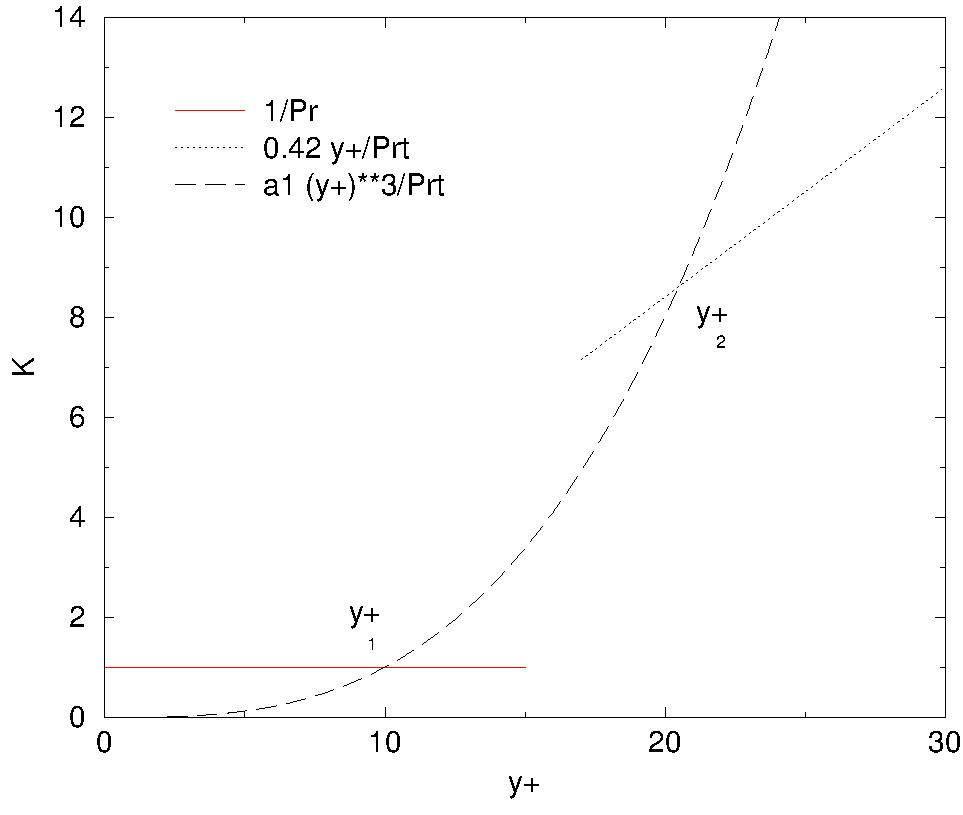
\includegraphics[height=8cm]{clthermique}}
\caption{$(a+a_t)/\nu$ as a function of $y^+$ obtained
                       for $\sigma=1$ and $\sigma_t=1$.}
\end{figure}


The values of $y^+_1$ and $y^+_2$ are obtained by calculating
the intersection points of the variations laws used
for $\mathcal{K}$.

The existence of an intermediate region depends upon the
values of $\sigma$.
Let's first consider the case where $\sigma$ cannot be neglected
compared to 1. In practise we consider  $\sigma > 0,1$
(this is the common case when scalar $f$ represents
the air or the water temperature in normal temperature
and pressure conditions). It is assumed that
$\displaystyle\frac{1}{\sigma}$ can be neglected compared to
$\displaystyle\frac{a_1 (y^+)^3}{\sigma_t}$ in the
intermediate region.
We thus obtain~:
\begin{equation}
  y^+_1 =\left(\displaystyle\frac{1000}{\sigma}\right)^\frac{1}{3} \qquad\qquad
  y^+_2 = \sqrt{\displaystyle\frac{1000\kappa}{\sigma_t}}
\end{equation}
The dimensionless equation~(\ref{Base_Clptur_Eq_Flux_scalaire_adim})
is integrated under the same hypothesis and we obtain the law of $f^+$~:
\begin{equation}
\left\{
\begin{array}{ll}
f^+ = \sigma \,y^+ & \text{if } y^+ < y^+_1 \\
f^+ = a_2 -\displaystyle\frac{\sigma_t}{2\,a_1\,(y^+)^2}& \text{if } y_1^+ \leqslant y^+ < y_2^+ \\
f^+ = \displaystyle\frac{\sigma_t}{\kappa}\,ln(y^+)+a_3& \text{if } y^+_2 \leqslant y^+\\
\end{array}
\right.
\end{equation}
where $a_2$ and $a_3$ are integration constants,
which have been chosen to obtain
a continuous  profile of $f^+$~:
\begin{equation}
a_2=15\sigma^{\frac{2}{3}}\qquad\qquad
a_3=15\sigma^{\frac{2}{3}}-\displaystyle\frac{\sigma_t}{2\kappa}
\left(1+
ln\left(\displaystyle\frac{1000\kappa}{\sigma_t}\right)\right)
\end{equation}

Let's now study the case where  $\sigma$ is much smaller than 1.
In practise it is assumed that $\sigma \leqslant 0,1$ (this is for
instance the case for liquid metals whose thermal conductivity is very
large, and who have Prandtl number of values of the order of 0.01).
The intermediate region then disappears and the coordinate of the
interface between the law used in the near-wall region and the one
used away from the wall is given by~:
\begin{equation}
y^+_0= \displaystyle\frac{\sigma_t}{\kappa\sigma}
\end{equation}

The dimensionless equation~(\ref{Base_Clptur_Eq_Flux_scalaire_adim})
is then integrated under the same hypothesis, and the law of
 $f^+$ is obtained~:
\begin{equation}
\left\{
\begin{array}{ll}
f^+ = \sigma \,y^+ & \text{if } y^+ \leqslant y^+_0 \\
f^+ = \displaystyle\frac{\sigma_t}{\kappa}\,
        ln\left(\displaystyle\frac{y^+}{y^+_0}\right)+\sigma \,y^+_0
                   & \text{if } y^+_0 < y^+\\
\end{array}
\right.
\end{equation}


\newpage
To summarize, the computation of $h_b$
\begin{equation}
h_b=\displaystyle\frac{\phi_b}{f_{b,ext}-f_{I'}}=\frac{\rho\,C\,u_k}{f^+_{I'}}
\end{equation}
is performed by calculating  $f^+_{I'}$ from $y^+=y^+_{I'}$
using the following laws.

If $\sigma\leqslant 0,1$, a two-layer model is used~:
\begin{equation}
\left\{
\begin{array}{ll}
f^+ = \sigma \,y^+ & \text{if } y^+ \leqslant y^+_0 \\
f^+ = \displaystyle\frac{\sigma_t}{\kappa}\,
        ln\left(\displaystyle\frac{y^+}{y^+_0}\right)+\sigma \,y^+_0
                   & \text{if } y^+_0 < y^+\\
\end{array}
\right.
\end{equation}
with
\begin{equation}
y^+_0= \displaystyle\frac{\sigma_t}{\kappa\sigma}
\end{equation}


If $\sigma > 0,1$, a three-layer model is used~:
\begin{equation}
\left\{
\begin{array}{ll}
f^+ = \sigma \,y^+ & \text{if } y^+ < y^+_1 \\
f^+ = a_2 -\displaystyle\frac{\sigma_t}{2\,a_1\,(y^+)^2}& \text{if } y_1^+ \leqslant y^+ < y_2^+ \\
f^+ = \displaystyle\frac{\sigma_t}{\kappa}\,ln(y^+)+a_3& \text{if } y^+_2 \leqslant y^+\\
\end{array}
\right.
\end{equation}
with
\begin{equation}
  y^+_1 =\left(\displaystyle\frac{1000}{\sigma}\right)^\frac{1}{3} \qquad\qquad
  y^+_2 = \sqrt{\displaystyle\frac{1000\kappa}{\sigma_t}}
\end{equation}
and
\begin{equation}
a_2=15\sigma^{\frac{2}{3}}\qquad\qquad
a_3=15\sigma^{\frac{2}{3}}-\displaystyle\frac{\sigma_t}{2\kappa}
\left(1+
ln\left(\displaystyle\frac{1000\kappa}{\sigma_t}\right)\right)
\end{equation}

\newpage
%%%%%%%%%%%%%%%%%%%%%%%%%%%%%%%%%%
%%%%%%%%%%%%%%%%%%%%%%%%%%%%%%%%%%
\section*{Points to treat}
%%%%%%%%%%%%%%%%%%%%%%%%%%%%%%%%%%
%%%%%%%%%%%%%%%%%%%%%%%%%%%%%%%%%%


The use of \var{HFLUI/CPP} when \var{ISCSTH} is 2 (case with
radiation) needs to be checked (\var{CPP} is actually 1 in this case).

The boundary conditions of the velocity are based on derivations
focusing on only one term of the tangential stress
$(\mu_I+\mu_{t,I})(\ggrad{\vect{u}})\,\vect{n}$ without taking
into account the tranpose gradient.

In order to establish the boundary conditions of the velocity in
$k-\varepsilon$ based on the constraint , a projection onto the plane
tangent to the wall and an arbitrary zero normal velocity
are introduced.

The hypothesis made in order to establish formulae for the different types
of boundary conditions (dissipation, velocities) are based on the assumption
that the mesh is orthogonal at the wall. This assumption is extended
without any caution to the case of non-orthogonal meshes.

The one velocity scale (\fort{cs\_wall\_functions.c}) wall function requires
solving an equation using a Newton algorithm.
The computational cost of the latter is low. One can also used
a  $1/7$ power law (Werner et Wengle) which yields results which are as
accurate as the logarithmic law in the logarithmic region, and which permits
analytical resolutions (chosen option in LES mode). Be careful however,
since with this law, the intersection with the linear law is
slightly different, which thus requires some adaptations (intersection
around 11.81 instead of 10.88 for the law adopted here
$U^+=8,3\,(y^+)^\frac{1}{7}$).


The values of all the physical properties are taken at the cell centres,
without any reconstruction. Without modifying this approach, it would be
useful to keep this in mind.

%
%
%
%Pb de continuite si YPLULI.NE.10.88
%
% Le mode de r\'esolution permettant d'obtenir $u^*$ est particulier. Avec le
%mod\`ele \`a une \'echelle de vitesse, on \'evalue
%tout d'abord la vitesse de frottement $u^*$ issue de la loi logarithmique. On
%pose $u_k=u^*$, puis on calcule la valeur de $y^+$.  Avec le
%mod\`ele \`a deux \'echelles, on calcule tout d'abord $u_k$, on en d\'eduit
%$y^+$ puis $u^*$. Dans les deux cas, si
%$y^+\leqslant y^+_{lim}=\displaystyle\frac{2}{\kappa}$, on applique une condition
%d'adh\'erence (vitesse impos\'ee nulle \`a la paroi, \'energie turbulente et
%tensions de Reynolds impos\'ees nulles, flux nul pour la dissipation).
%Il serait bon de v\'erifier que cette m\'ethode, qui utilise une loi
%logarithmique jusqu'\`a de tr\`es petites
%valeurs de $y^+$, ne conduit pas \`a des valeurs trop faibles de la
%vitesse de frottement lorsqu'on s'approche de la paroi ($y^+ \leqslant 10$).
%La figure \ref{Base_Clptur_fig_loi_log_clptur} propose une illustration~: supposons qu'en un
%point on obtienne, avec la m\'ethode actuelle, $u+\approx 8,6$ et
%$y^+\approx 4,3$. On en d\'eduit alors que la vitesse de frottement est
%$u^*\approx 1$ (courbe logarithmique en trait plein (noire) repr\'esentant
%$ln(y^+)/0,42+5,2$).
%Toutes choses \'egales par ailleurs (ce qui constitue une
%hypoth\`ese en soi), avec une m\'ethode prenant en compte une loi lin\'eaire en
%dessous de $y^+\approx 10$, on aurait obtenu $u^*\approx 2$
%(courbe lin\'eaire en trait plein (rouge) repr\'esentant $2y^+$). Bien
%entendu, cette analyse est relativement na\"\i ve et ne prend pas en compte le
%caract\`ere implicite des r\'esolutions ainsi que le fait qu'il est d'ordinaire
%peu recommand\'e de placer la premi\`ere maille \`a des valeurs aussi faibles de
%$y^+$ avec les mod\`eles de type haut Reynolds.
%
%\begin{figure}[h]
%\centerline{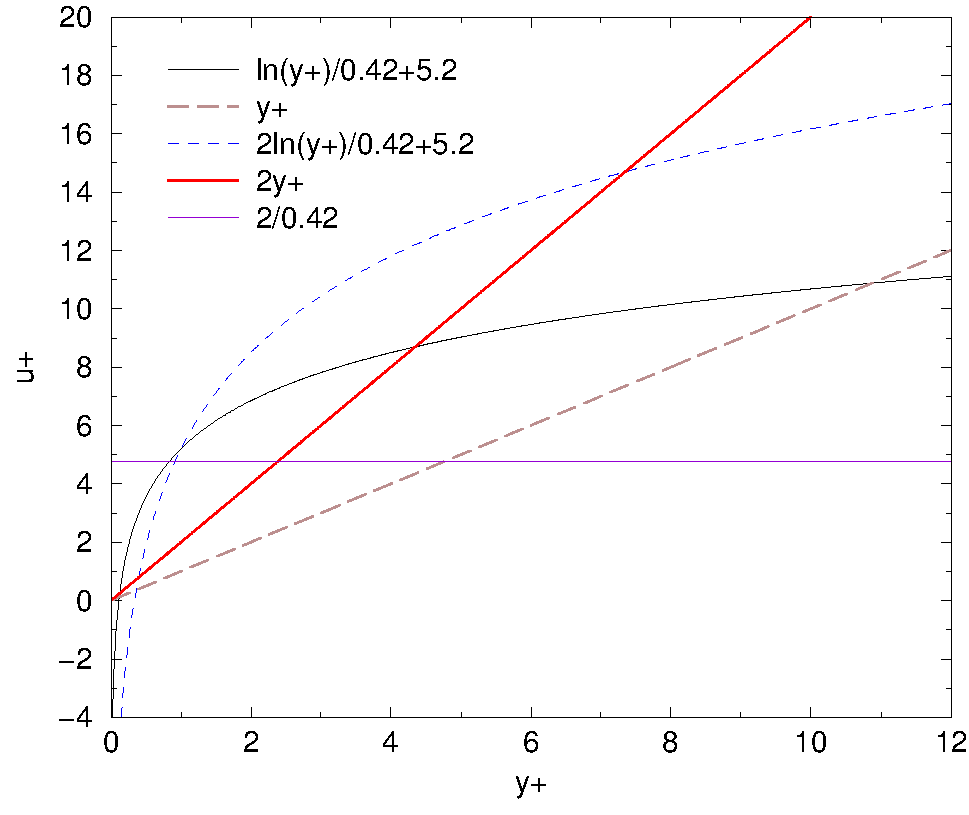
\includegraphics[height=7cm]{loilog}}
%\caption{\label{Base_Clptur_fig_loi_log_clptur}D\'etermination de $y^+$.}
%\end{figure}



% Plus d'actualite a priori, mais pistes de reflexion quand meme
%La limitation par valeur minimale de la vitesse dans (\ref{Base_Clptur_eq_ugrad_clptur})
%a \'et\'e corrig\'ee dans la version 1.1.0.q.
%Auparavant, la formulation \'etait susceptible de conduire
%\`a une valeur trop faible du gradient de vitesse et donc de la production
%turbulente en paroi. Elle s'\'ecrivait~:
%\begin{equation}
%u_{\tau,F,grad} =u_{\tau,I'}-\displaystyle\frac{u^*}{\kappa}min\left[max\left(1,
%2\sqrt{\displaystyle\frac{\rho_I\kappa\, u_k I'F}{\mu_{t,I}}
%}-\displaystyle\frac{1}{2}\right),ln\frac{2}{\kappa}+5,2\kappa\right]
%\end{equation}
%La  formulation a \'et\'e modifi\'ee~:
%\begin{equation}\notag
%u_{\tau,F,grad} =max\left(u^*(\frac{1}{\kappa}ln\displaystyle\frac{2}{\kappa}+5,2),
%u_{\tau,I'}-\displaystyle\frac{u^*}{\kappa}\left[max\left(1,
%2\sqrt{\displaystyle\frac{\rho_I\kappa\, u_k I'F}{\mu_{t,I}}
%}-\displaystyle\frac{1}{2}\right)\right]\right)
%\end{equation}
%Elle a \'et\'e adopt\'ee apr\`es des tests sur des
%configurations de validation (canal, marche descendante,  jet impactant, dune,
%echo, rra) qui n'ont montr\'e aucune influence de la modification.
%\`A partir de la version 1.1.0.t, on a utilis\'e la valeur
%$y^+_\text{lim}=10,88$ et non plus $\frac{2}{\kappa}$ pour caract\'eriser le
%passage de la loi lin\'eaire \`a la loi logarithmique et la
%relation a donc \'et\'e modifi\'ee comme suit~:
%\begin{equation}\notag
%u_{\tau,F,grad} =max\left(u^*(\frac{1}{\kappa}ln(y^+_\text{lim})+5,2),
%u_{\tau,I'}-\displaystyle\frac{u^*}{\kappa}\left[max\left(1,
%2\sqrt{\displaystyle\frac{\rho_I\kappa\, u_k I'F}{\mu_{t,I}}
%}-\displaystyle\frac{1}{2}\right)\right]\right)
%\end{equation}
%Comme, pour des $y^+$ inf\'erieurs \`a $y^+_\text{lim}$, on applique une
%condition d'adh\'erence, cette approche n'est pas continue au voisinage de
%$y^+_\text{lim}$. Il serait utile de se pencher sur la question.
%Il faut cependant garder \`a l'esprit que la condition
%de Dirichlet pour $k$ est prise nulle quand  $y^+$ est inf\'erieur \`a
%$y^+_\text{lim}$, ce qui tend \'egalement  \`a annuler la production,
%quelle que soit la condition \`a la limite utilis\'ee pour la vitesse.


For the thermal law with very small Prandtl numbers compared to 1,
Arpaci and Larsen suggest $y_0^+ \simeq 5/Pr$ (with proof from
experimental data) rather than $Pr_t/(Pr\,\kappa)$  (current value,
computed as the analytical intersection of the linear and logarithmic
laws considered). One should address this question.


